\documentclass[journal]{IEEEtran}
\usepackage[a5paper, margin=10mm, onecolumn]{geometry}
%\usepackage{lmodern} % Ensure lmodern is loaded for pdflatex
\usepackage{tfrupee} % Include tfrupee package

\setlength{\headheight}{1cm} % Set the height of the header box
\setlength{\headsep}{0mm}     % Set the distance between the header box and the top of the text

\usepackage{gvv-book}
\usepackage{gvv}
\usepackage{cite}
\usepackage{amsmath,amssymb,amsfonts,amsthm}
\usepackage{algorithmic}
\usepackage{graphicx}
\usepackage{textcomp}
\usepackage{xcolor}
\usepackage{txfonts}
\usepackage{listings}
\usepackage{enumitem}
\usepackage{mathtools}
\usepackage{gensymb}
\usepackage{comment}
\usepackage[breaklinks=true]{hyperref}
\usepackage{tkz-euclide} 
\usepackage{listings}
% \usepackage{gvv}                                        
\def\inputGnumericTable{}                                 
\usepackage[latin1]{inputenc}                                
\usepackage{color}                                            
\usepackage{array}                                            
\usepackage{longtable}                                       
\usepackage{calc}                                             
\usepackage{multirow}                                         
\usepackage{hhline}                                           
\usepackage{ifthen}                                           
\usepackage{lscape}
\begin{document}

\bibliographystyle{IEEEtran}
\vspace{3cm}

\title{10.3.2.4.4}
\author{EE24BTECH11024 - G. Abhimanyu Koushik}
 \maketitle
% \newpage
% \bigskip
{\let\newpage\relax\maketitle}

\renewcommand{\thefigure}{\theenumi}
\renewcommand{\thetable}{\theenumi}
\setlength{\intextsep}{10pt} % Space between text and floats


\numberwithin{equation}{enumi}
\numberwithin{figure}{enumi}
\renewcommand{\thetable}{\theenumi}


\textbf{Question}:\\
Check is the pair of linear equations $2x-2y-2=0$, $4x-4y-5=0$. And if consistent, obtain the solution
\\
\textbf{Solution: }\\
Given
\begin{align}
    2x-2y-2=0\\
    4x-4y-5 = 0
\end{align}
Simplifying and using matrix notation,
\begin{align}
    \myvec{
        1 & -1\\
        4 & -4
    } \myvec{x \\ y}= \myvec{ 1 \\ 5}
\end{align}
The matrix $A$ can be decomposed into:
\begin{align}
    A = L \cdot U,
\end{align}
where:
\begin{align}
    L &= \myvec{1 & 0 \\ 4 & 1}, \\
    U &= \myvec{1 & -1 \\ 0 & 0}.
\end{align}
\newline
Factorization of LU:\newline
Given a matrix $ \mathbf{A} $ of size $ n \times n $, LU decomposition is performed row by row and column by column. The update equations are as follows: \\ 
\qquad 1. Start by initializing $ \mathbf{L} $ as the identity matrix $ \mathbf{L} = \mathbf{I} $ and $ \mathbf{U} $ as a copy of $ \mathbf{A} $.\\
\qquad 2. For each column $ j \geq k $, the entries of $ U $ in the $ k $-th row are updated as:
\begin{align}
U_{k,j} = A_{k,j} - \sum_{m=1}^{k-1} L_{k,m} \cdot U_{m,j}\quad \forall \quad j \geq k
\end{align}
3. For each row $ i > k $, the entries of $ L $ in the $ k $-th column are updated as:
\begin{align}
L_{i,k} = \frac{1}{U_{k,k}} \brak{ A_{i,k} - \sum_{m=1}^{k-1} L_{i,m} \cdot U_{m,k}} \quad \forall \quad i > k
\end{align}
The system $A\vec{x} = \vec{b}$ is transformed into $L \cdot U \cdot \vec{x} = \vec{b}$. Let $\vec{y}$ satisfy $L\vec{y} = \vec{b}$:
\begin{align}
    \myvec{1 & 0 \\ 4 & 1} \myvec{y_1 \\ y_2} = \myvec{1 \\ 5}.
\end{align}
Using forward substitution:
\begin{align}
    y_1 &= 1 \\
    4y_1 + y_2 &= 5\\
    y_2 &= 1
\end{align}
Thus:
\begin{align}
    \vec{y} = \myvec{1 \\ 1}.
\end{align}

Next, solve $U\vec{x} = \vec{y}$:
\begin{align}
    \myvec{1 & -1 \\ 0 & 0} \myvec{x \\ y} = \myvec{1 \\ 1}.
\end{align}

Using back substitution:
\begin{align}
	0x+0y = 1
\end{align}
As it is not possible for any value of $x$ and $y$, the solution does not exist.

\begin{figure}[h!]
   \centering
   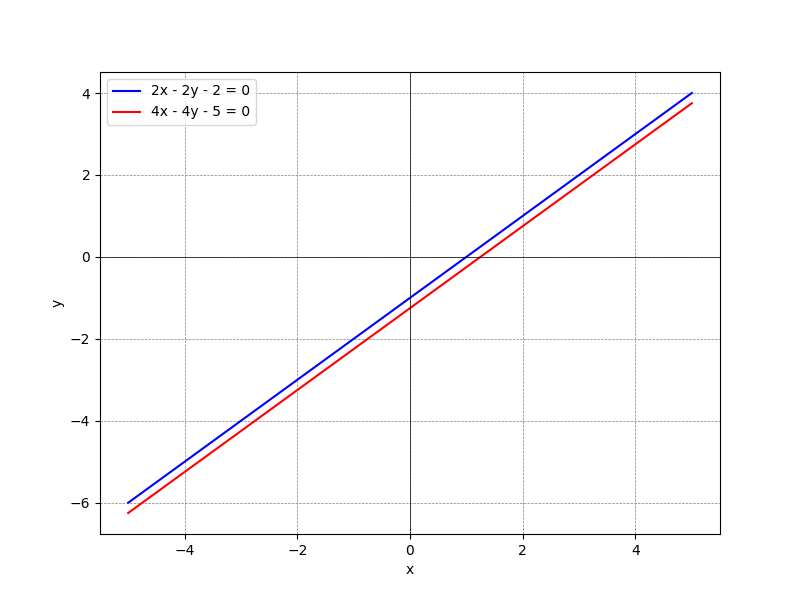
\includegraphics[width=1\columnwidth]{figs/fig.png}
    \caption{Solution to set of linear equations}
\end{figure}
\end{document}
